% ============================================================
% 4  Stretched exponential in the electron (large-N prediction, flashed)
% ============================================================
\begin{frame}[t]
\ft{Stretched exponential in the electron}\par
\vspace{0.4cm}
\begin{columns}[c]
\begin{column}{0.60\textwidth}
\centering
\onslide<2->{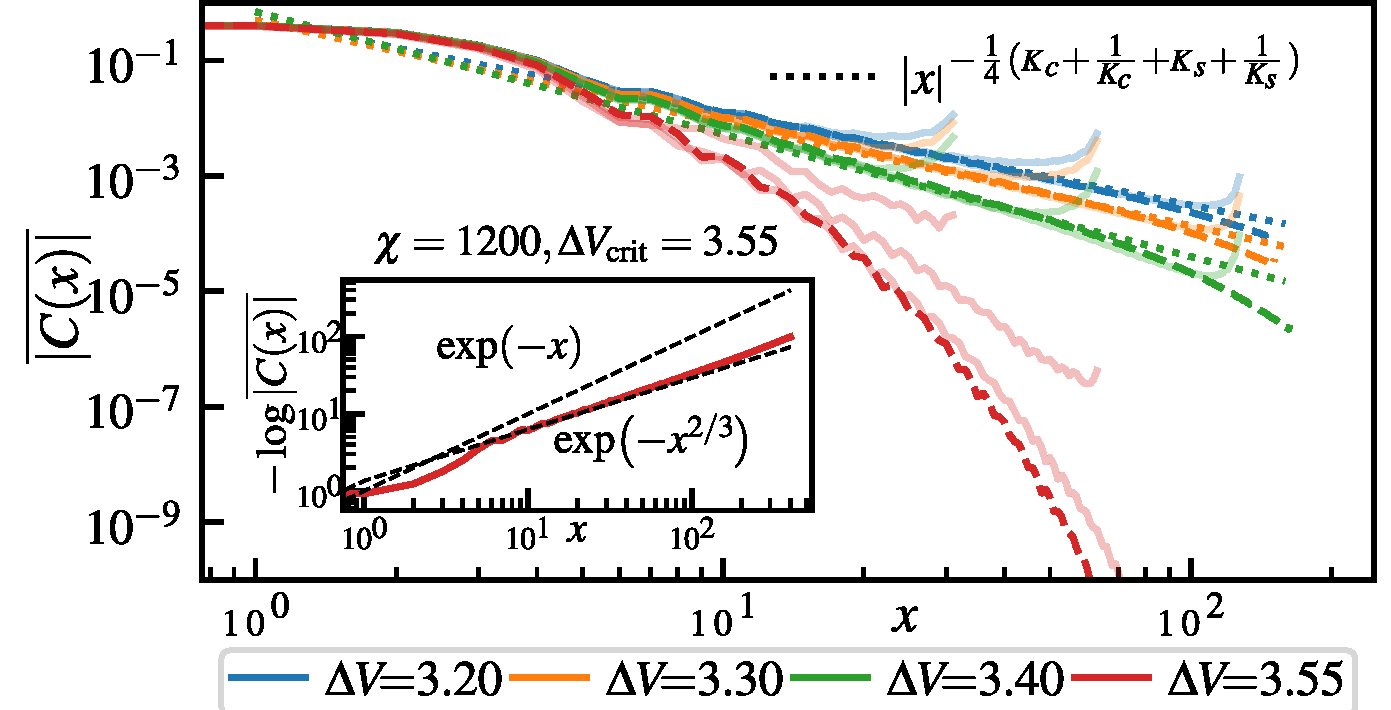
\includegraphics[width=\linewidth]{figures/paper_fig1_green.png}\par}
\end{column}
\begin{column}{0.38\textwidth}
{\small $\theta$ stiff $\Rightarrow$ its conjugate $\phi_s$ fluctuates wildly\par}
\vspace{0.2cm}
\colorbox{cQCP!15}{\mystrut large-$N$ theory}:\\[2pt]
\hspace*{0.3cm}{\footnotesize$\langle e^{i\phi_x}e^{-i\phi_0}\rangle\sim e^{-c\,x^{2/3}}$\par}
{\tiny\color{citegray} large-$N$ saddle point:\\ Andriyakhina, Shankar, Senthil, Shi (2026)\par}
\vspace{0.3cm}
\onslide<2->{{\small $c_{\uparrow}\sim e^{i\sqrt{\pi/2}\,(\phi_c+{\color{cQCP}\phi_s}+\theta_c+\theta_s)}$\par}
{\footnotesize the electron contains $\phi_s$\par}
\vspace{0.1cm}
\colorbox{cLL!20}{\mystrut Luttinger liquid}: {\footnotesize power laws\par}}
\vspace{0.3cm}
\onslide<3->{\colorbox{cQCP!15}{\mystrut Critical point}:\\[2pt]
\hspace*{0.3cm}$C(x)\sim e^{-c\,x^{2/3}}$\\[2pt]
\hspace*{0.3cm}{\footnotesize inset: slope close to $2/3$\par}}
\end{column}
\end{columns}
\onslide<3->{\tk{Large-$N$ prediction seen at $N=1$}}
\end{frame}
% Notes: The large-N calculation is the co-authors' work; only its result is flashed here (saddle point of the large-N theory, paper and backup). Step 1: theta is stiff, so its conjugate phi_s fluctuates wildly; large N predicts a stretched exponential exp(-c x^{2/3}) for the phi_s vertex.
% Notes: Step 2: The electron itself contains the conjugate spin vertex e^{i phi_s}, so the prediction should show up in the single-electron Green's function C(x) (averaged over 4 sites to remove the k_F Friedel oscillations). In the LL phase (blue, orange, green) all channels are power laws, envelope |x|^{-1/4(K_c+1/K_c+K_s+1/K_s)}.
% Notes: Step 3: At the QCP (red) the decay turns over to faster than any power law. Inset: -log C vs x on log-log: slope close to 2/3, clearly below the pure exponential. The fitted slope moves toward 2/3 with increasing bond dimension (finite-entanglement scaling, supplement). The qualitative large-N prediction holds already at N = 1.
